\section{Funzioni in più variabili}
\begin{equation}
    f: \underset{(x_1, \, \dotsc, \, x_n)}{A \subseteq \R^n} \underset{\mapsto}{\to} \underset{f(x_1, \, \dotsc, \, x_n)}{\R}
\end{equation}

\begin{definition}[Funzione scalare]
    Viene detta \emph{FUNZIONE SCALARE (VETTORIALE)} di più variabili una funzione
    \begin{equation}
        f: \Omega \to \R  \mbox{ con } \Omega \subseteq \R^n \; (n>1)
    \end{equation}
\end{definition}

\subsection{Limiti}
\underline{\textbf{Risoluzione:}}
\begin{enumerate}
    \item \textbf{Trovare un candidato limite} \\
    Segliere restrizioni facili per determinare il candidato\\
    \es $\mspace{10mu} \lim_{(x,y) \to (0,0)}$ posso usare gli assi come restrizione:
    \[ \lim_{x \to 0} f(x,0) = l \] \[ \lim_{y \to 0} f(0, y) = l \]
    e $l$ sarà il candidato.

    \item \textbf{Verificare che il limite sia uguale al candidato su altre restrizioni}\\
    $lim_{(x,y) \to (x_0, y_0)}$, si usano restrizioni del tipo
    \[ y-y_0 = m(x-x_0)^\alpha \mspace{25mu} \alpha > 0\]
    che sono rette, parabole ecc.\\
    \es \space restrizione con parabola:
    \[ \lim_{(x,y) \to (x_0, y_0)} f(x, mx^2) \]

    \item \textbf{Esistenza del limite}\\
    Ci sono due modi:
    \begin{itemize}
        \item Maggiorazioni
        \[ |f(x, y) - l| \leq \varepsilon, \mspace{25mu} \varepsilon \to 0 \]
        \item Coordinate polari
        \[ \begin{cases}
            x = \rho \cos\theta \\
            y = \rho \sin\theta
        \end{cases}\]
        \begin{theorem}
            Esiste $\lim_{(x,y) \to (x_0, y_0)} f(x,y) = l$ se e solo se esistono $r>0$ e $g:(0, r) \to \R$ tali che 
            \begin{itemize}
                \item [$i$)] \[ |f(x_0 + \rho \cos \theta, y_0 + \rho \sin\theta) - l | \leq g(\rho) \]
                per ogni $\rho \in (0, r)$ ed ogni $\theta \in [0, 2\pi)$

                \item [$ii$)] \[ \lim_{\rho \to 0^+} g(\rho) = 0 \]
            \end{itemize}
        \end{theorem}
    \end{itemize}
\end{enumerate}

\subsection{Derivate parziali e gradiente}
In $\R^2$:

\begin{definition}[Derivate parziali]
    Sia $f : \underset{\mbox{\scriptsize{aperto}}}{A} \subseteq \R^2 \to \R$, con $(x_0, y_0) \in A$, si dicono \emph{DERIVATE PARZIALI} di $f$ in $(x_0, y_0)$
    \begin{equation}
        \frac{\partial f}{\partial x}(x_0, y_0) \mspace{25mu} \mbox{o} \mspace{25mu} f_x(x_0, y_0)
    \end{equation}
    \begin{equation}
        \frac{\partial f}{\partial y}(x_0, y_0) \mspace{25mu} \mbox{o} \mspace{25mu} f_y(x_0, y_0)
    \end{equation}
\end{definition}

\underline{\textbf{Risoluzione:}}\\
Si calcolano come derivate dell'Analisi 1: nel caso di $\frac{\partial f}{\partial x}$ si calcola la derivata rispetto a $x$, trattando $y$ come se fosse un parametro.\\

\es \\
$f(x, y) = x^2 y + \sin(x^3)$
\[ \frac{\partial f}{\partial x} = 2xy + 3x^2 \sin(x^3) \]
\[ \frac{\partial f}{\partial y} = x^2 \]

\subsubsection{Gradiente}
\begin{definition}[Gradiente]
    Si dice \emph{GRADIENTE} di $f$ in $(x_0, y_0)$ il vettore
    \begin{equation}
        \nabla f(x_0, y_0) = \left( \frac{\partial f}{\partial x}(x_0, y_0), \; \frac{\partial f}{\partial y}(x_0, y_0) \right)
    \end{equation}
\end{definition}

\underline{\textbf{Risoluzione:}}\\
Si devono calcolare le singole derivate parziali
\[
    \nabla f(x_0, y_0) = 
    \begin{cases}
        \frac{\partial f}{\partial x}(x_0, y_0)\\
        \frac{\partial f}{\partial y}(x_0, y_0)
    \end{cases}
\]

\subsubsection{Derivate direzionali e formula del gradiente}
Sia $\vec{v}$ un vettore t.c $|| \vec{v} || = 1$.\\
Una derivata direzionale lungo una direzione $\vec{v}$ in un punto $(x_0, y_0)$ è
\begin{equation}
    \partial_{\vec{v}} f (x_0, y_0) = \lim_{t \to 0} \frac{f(x_0 + \vec{v}_x  t, \; y_0 + \vec{v}_y  t) - f(x_0, y_0)}{t}
\end{equation}

Se $f$ è differenziabile in $(x_0, y_0)$, vale la \emph{FORMULA DEL GRADIENTE}
\begin{equation}
    \partial_{\vec{v}} f (x_0, y_0) = \,< \nabla f(x_0, y_0) ,    \; \vec{v} >
\end{equation}

\subsubsection{Differenziabilità}
Una funzione $f : \underset{\mbox{\scriptsize{aperto}}}{A} \subseteq \R^2 \to \R$ è \emph{DIFFERENZIABILE} in $(x_0, y_0) \in A$ se e solo se
\begin{enumerate}
    \item Esistono le derivate parziali in $(x_0, y_0)$ (esiste $\nabla f (x_0, y_0) \in \R^2$)
    \item \[ \lim_{(h,k)\to (0,0)} \frac{f(x_0 + h, \; y_0 + k) - f(x_0, \;y_0) - \frac{\partial f}{\partial x} (x_0, \; y_0) \cdot h - \frac{\partial f}{\partial y} (x_0, \; y_0) \cdot k}{\sqrt{h^2 + k^2}} = 0  \]
\end{enumerate}

\subsection{Ottimizzazione}
Ricerca di punti di massimo e di minimo realtivi e assoluti\\

\underline{\textbf{Risoluzione:}}
\begin{enumerate}
    \item Ricerca dei punti critici \\
    \[ \nabla f (x,\,y) = (0,0)  \]
    \[
        \begin{cases}
            \frac{\partial f}{\partial x}= 0\\
            \frac{\partial f}{\partial y}= 0
        \end{cases}
    \]

    \item Scrittura della martice Hessiana:
    \begin{equation}
        H_f(x, \, y) = \left[
            \begin{array}{c c}
                \frac{\partial^2 f}{\partial x^2}(x, \, y)  & \frac{\partial^2 f}{\partial x \partial y}(x, \, y) \\ \\
                \frac{\partial^2 f}{\partial x \partial y}(x, \, y) & \frac{\partial^2 f}{\partial y^2}(x, \, y)
            \end{array}
        \right]
    \end{equation}

    \item Classificazione dei punti critici:
    \begin{theorem}[Criterio dell'Hessiana]
        Sia $f : \underset{\mbox{\scriptsize{aperto}}}{A} \subseteq \R^2 \to \R$ di classe $C^2 (A)$ e sia $(x_0, \; y_0) \in A$ punrio critico per $f$.\\
        Allora
        \begin{itemize}
            \item [$i$)] Se tutti gli autovalori di $H_f (x_0,\, y_0)$ sono $> 0$, $(x_0, \; y_0)$ è punto di \emph{MINIMO RELATIVO}
            \begin{center}
                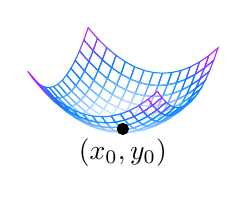
\begin{tikzpicture} 
                    \begin{axis}[
                        colormap/cool,
                        hide axis,
                        width = 4cm,
                        clip = false,
                        %axis lines=center, axis on top,
                        %axis line style = {gray}
                        %xtick=\empty, ytick=\empty,ztick=\empty,
                        ]
                        \addplot3 [
                            domain=-5:5,
                            domain y = -5:5,
                            samples = 15,
                            samples y = 15,
                            mesh,
                            width = 3cm,
                        ] {x^2 + y^2};

                        \addplot3 [
                            mark = *,
                            black
                        ]coordinates {(0,0,0)} node[anchor=north]{$(x_0, y_0)$};
                    \end{axis}                 
                \end{tikzpicture}
            \end{center}
            \item [$ii$)] Se tutti gli autovalori di $H_f (x_0,\, y_0)$ sono $< 0$, $(x_0, \; y_0)$ è punto di \emph{MASSIMO RELATIVO}
            \begin{center}
                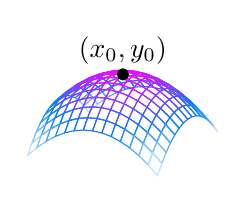
\begin{tikzpicture} 
                    \begin{axis}[
                        colormap/cool,
                        hide axis,
                        width = 4cm,
                        clip = false
                        ]
                        \addplot3 [
                            domain=-5:5,
                            domain y = -5:5,
                            samples = 15,
                            samples y = 15,
                            mesh,
                            width = 3cm,
                        ] {- (x^2 + y^2)};

                        \addplot3 [
                            mark = *,
                            black
                        ]coordinates {(0,0,0)} node[anchor=south]{$(x_0, y_0)$};
                    \end{axis}                 
                \end{tikzpicture}
            \end{center}
            \item [$iii$)] Se $\exists \lambda_1, \, \lambda_2$ autovalori di $H_f (x_0,\, y_0)$ discordi, $(x_0, \; y_0)$ è punto di \emph{SELLA}
            \begin{center}
                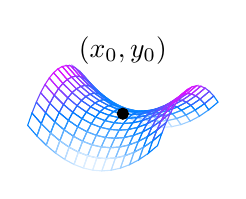
\begin{tikzpicture} 
                    \begin{axis}[
                        colormap/cool,
                        hide axis,
                        width = 4cm,
                        clip=false
                        ]
                        \addplot3 [
                            domain=-5:5,
                            domain y = -5:5,
                            samples = 15,
                            samples y = 15,
                            mesh,
                            width = 3cm,
                        ] {x^2 - y^2)};

                        \addplot3 [
                            mark = *,
                            black
                        ]coordinates {(0,0,0)} node[anchor=south, yshift=.5cm]{$(x_0, y_0)$};
                    \end{axis}                 
                \end{tikzpicture}
            \end{center}
            \item [$iv$)] In tutti gli altri casi serve un'analisi ulteriore.
        \end{itemize}
        \label{hess}
    \end{theorem}

    \underline{In $\R^2$}, dato che serve conoscere solo il segno degli autovalori, basta studiare il segno del determinante dell'Hessiana:
    \begin{itemize}[topsep=0pt]
        \item Se $det(H_f (x_0,\, y_0)) < 0$, gli autovalori sono discordi e $(x_0, \; y_0)$ è un punto di sella 
        \item Se $det(H_f (x_0,\, y_0)) > 0$, gli autovalori sono concordi ed il segno è determinato dal primo elemento della matrice (metodo dei minimi da nord-ovest):
        \begin{itemize}[topsep=0pt]
            \item se $f_{xx} (x_0, \; y_0) < 0$, $(x_0, \; y_0)$ è un punto di massimo relativo
            \item se $f_{xx} (x_0, \; y_0) > 0$, $(x_0, \; y_0)$ è un punto di minimo relativo
        \end{itemize}
    \end{itemize}

    nel caso di uno o più autovalori nulli (punto $iv$ del Criterio dell'Hessiana (\ref{hess}))
    %?????????????????????????????

    \item Ricerca dei punti di massimo e minimo assoluti:\\
    è necessario studiare il segno di
    \begin{equation}
        \Delta f(x, \, y) = f(x,\, y) - f(x_0, \, y_0)
    \end{equation}
    \begin{itemize}
        \item Se $\Delta f \leq 0, \; \forall\, (x, \, y) \in D$, $(x_0, \; y_0)$ è punto di massimo assoluto o globale
        \item Se $\Delta f \geq 0, \; \forall\, (x, \, y) \in D$, $(x_0, \; y_0)$ è punto di minimo assoluto o globale
    \end{itemize}
\end{enumerate}
